\documentclass[journal,12pt,twocolumn]{IEEEtran}

\usepackage{setspace}
\usepackage{gensymb}
\singlespacing
\usepackage[cmex10]{amsmath}

\usepackage{amsthm}
\usepackage{commath}
\usepackage{mathrsfs}
\usepackage{txfonts}
\usepackage{stfloats}
\usepackage{bm}
\usepackage{cite}
\usepackage{cases}
\usepackage{subfig}

\usepackage{longtable}
\usepackage{multirow}

\usepackage{enumitem}
\usepackage{mathtools}
\usepackage{steinmetz}
\usepackage{tikz}
\usepackage{circuitikz}
\usepackage{verbatim}
\usepackage{tfrupee}
\usepackage[breaklinks=true]{hyperref}
\usepackage{graphicx}
\usepackage{tkz-euclide}

\usetikzlibrary{calc,math}
\usepackage{listings}
    \usepackage{color}                                            %%
    \usepackage{array}                                            %%
    \usepackage{longtable}                                        %%
    \usepackage{calc}                                             %%
    \usepackage{multirow}                                         %%
    \usepackage{hhline}                                           %%
    \usepackage{ifthen}                                           %%
    \usepackage{lscape}     
\usepackage{multicol}
\usepackage{chngcntr}

\DeclareMathOperator*{\Res}{Res}

\renewcommand\thesection{\arabic{section}}
\renewcommand\thesubsection{\thesection.\arabic{subsection}}
\renewcommand\thesubsubsection{\thesubsection.\arabic{subsubsection}}

\renewcommand\thesectiondis{\arabic{section}}
\renewcommand\thesubsectiondis{\thesectiondis.\arabic{subsection}}
\renewcommand\thesubsubsectiondis{\thesubsectiondis.\arabic{subsubsection}}
\newtheorem{theorem}{Theorem}[section]
\newtheorem{corollary}{Corollary}[theorem]
\newtheorem{lemma}[theorem]{Lemma}
\newtheorem{definition}{Definition}[section]

\hyphenation{op-tical net-works semi-conduc-tor}
\def\inputGnumericTable{}                                 %%

\lstset{
%language=C,
frame=single, 
breaklines=true,
columns=fullflexible
}
\begin{document}

\newcommand{\BEQA}{\begin{eqnarray}}
\newcommand{\EEQA}{\end{eqnarray}}
\newcommand{\define}{\stackrel{\triangle}{=}}
\bibliographystyle{IEEEtran}
\raggedbottom
\setlength{\parindent}{0pt}
\providecommand{\mbf}{\mathbf}
\providecommand{\pr}[1]{\ensuremath{\Pr\left(#1\right)}}
\providecommand{\qfunc}[1]{\ensuremath{Q\left(#1\right)}}
\providecommand{\sbrak}[1]{\ensuremath{{}\left[#1\right]}}
\providecommand{\lsbrak}[1]{\ensuremath{{}\left[#1\right.}}
\providecommand{\rsbrak}[1]{\ensuremath{{}\left.#1\right]}}
\providecommand{\brak}[1]{\ensuremath{\left(#1\right)}}
\providecommand{\lbrak}[1]{\ensuremath{\left(#1\right.}}
\providecommand{\rbrak}[1]{\ensuremath{\left.#1\right)}}
\providecommand{\cbrak}[1]{\ensuremath{\left\{#1\right\}}}
\providecommand{\lcbrak}[1]{\ensuremath{\left\{#1\right.}}
\providecommand{\rcbrak}[1]{\ensuremath{\left.#1\right\}}}
\theoremstyle{remark}
\newtheorem{rem}{Remark}
\newcommand{\sgn}{\mathop{\mathrm{sgn}}}
\providecommand{\abs}[1]{\vert#1\vert}
\providecommand{\res}[1]{\Res\displaylimits_{#1}} 
\providecommand{\norm}[1]{\lVert#1\rVert}
%\providecommand{\norm}[1]{\lVert#1\rVert}
\providecommand{\mtx}[1]{\mathbf{#1}}
\providecommand{\mean}[1]{E[ #1 ]}
\providecommand{\fourier}{\overset{\mathcal{F}}{ \rightleftharpoons}}
%\providecommand{\hilbert}{\overset{\mathcal{H}}{ \rightleftharpoons}}
\providecommand{\system}{\overset{\mathcal{H}}{ \longleftrightarrow}}
	%\newcommand{\solution}[2]{\textbf{Solution:}{#1}}
\newcommand{\solution}{\noindent \textbf{Solution: }}
\newcommand{\cosec}{\,\text{cosec}\,}
\providecommand{\dec}[2]{\ensuremath{\overset{#1}{\underset{#2}{\gtrless}}}}
\newcommand{\myvec}[1]{\ensuremath{\begin{pmatrix}#1\end{pmatrix}}}
\newcommand{\mydet}[1]{\ensuremath{\begin{vmatrix}#1\end{vmatrix}}}
\numberwithin{equation}{subsection}
\makeatletter
\@addtoreset{figure}{problem}
\makeatother
\let\StandardTheFigure\thefigure
\let\vec\mathbf
\renewcommand{\thefigure}{\theproblem}
\def\putbox#1#2#3{\makebox[0in][l]{\makebox[#1][l]{}\raisebox{\baselineskip}[0in][0in]{\raisebox{#2}[0in][0in]{#3}}}}
     \def\rightbox#1{\makebox[0in][r]{#1}}
     \def\centbox#1{\makebox[0in]{#1}}
     \def\topbox#1{\raisebox{-\baselineskip}[0in][0in]{#1}}
     \def\midbox#1{\raisebox{-0.5\baselineskip}[0in][0in]{#1}}
\vspace{3cm}
\title{Assignment 5}
\author{Savarana Datta - AI20BTECH11008}
\maketitle
\newpage
\bigskip
\renewcommand{\thefigure}{\theenumi}
\renewcommand{\thetable}{\theenumi}
Download all python codes from 
\begin{lstlisting}
https://github.com/SavaranaDatta/EE3900/blob/main/EE3900_GATE_Assignment2/codes
\end{lstlisting}
%
Download latex-tikz codes from 
%
\begin{lstlisting}
https://github.com/SavaranaDatta/EE3900/blob/main/EE3900_GATE_Assignment2/GATE_Assignment2.tex
\end{lstlisting}
\section{Problem(GATE EC Q.32)}
The signal x(t) is described by 
\begin{align}
 x(t)=
\begin{cases}
1 & ,\text{for} -1 \leq t \leq +1\\
0 & ,otherwise
\end{cases} 
\end{align}
Two of the angular frequencies at which its fourier transform becomes zero are 
\begin{enumerate}
\item\label{1} $\pi$,2$\pi$
\item 0.5$\pi$,1.5$\pi$
\item 0,$\pi$
\item 2$\pi$,2.5$\pi$
\end{enumerate}
\section{Solution}
\begin{lemma}\label{eq}
The fourier transform of a rect function is sinc function 
\begin{align}
    rect\brak{\frac{t}{\tau}} \fourier \tau sinc\brak{f\tau}
\end{align}
\begin{proof}
\begin{align}
    \int_{-\infty}^{\infty} rect\brak{\frac{x}{\tau}} e^{-i2\pi xt} dx&= \int_{\frac{-\tau}{2}}^{\frac{\tau}{2}} e^{-i2\pi xt}dx\\
    &=\sbrak{\frac{e^{-i2\pi xt}}{-i2\pi t}}_{\frac{-\tau}{2}}^{\frac{\tau}{2}}\\
    &=\frac{e^{-i\pi t\tau}-e^{i\pi t\tau}}{-i2\pi t}\\
    &=\tau \frac{\sin{\pi t\tau}}{\pi t\tau}\\
    &=\tau sinc(t\tau)
\end{align} 
\end{proof}
\end{lemma}
We can observe that 
\begin{align}
    x(t)=rect(\frac{t}{2})
\end{align}
From the lemma \ref{eq}, fourier transform of x(t) is 
\begin{align}
    x(f)&= 2 sinc(2f)\\ 
        &= 2 \frac{sin\brak{2\pi f}}{\brak{2 \pi f}}\\
        &= 2 \frac{sin(\omega)}{\omega}
\end{align}
x(f) is zero when $\omega=n\pi$, where $n\in I-\{0\}$. Hence, option \ref{1} is true.
\begin{figure}[!h]
 \centering
 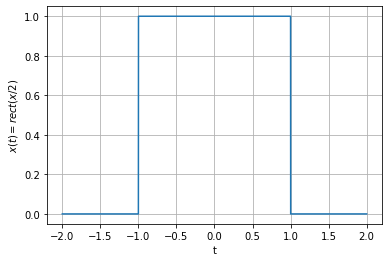
\includegraphics[width=\columnwidth]{rect.png}
 \caption{Plot of x(t)}
 \label{plot}
\end{figure}
\begin{figure}[!h]
 \centering
 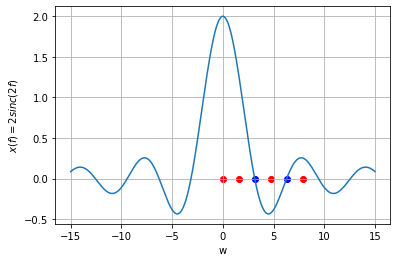
\includegraphics[width=\columnwidth]{sinc.png}
 \caption{Plot of the fourier transform}
 \label{plot}
\end{figure}
\end{document}

